\documentclass{book}
\usepackage[a4paper,top=2.5cm,bottom=2.5cm,left=2.5cm,right=2.5cm]{geometry}
\usepackage{makeidx}
\usepackage{natbib}
\usepackage{graphicx}
\usepackage{multicol}
\usepackage{float}
\usepackage{listings}
\usepackage{color}
\usepackage{ifthen}
\usepackage[table]{xcolor}
\usepackage{textcomp}
\usepackage{alltt}
\usepackage{ifpdf}
\ifpdf
\usepackage[pdftex,
            pagebackref=true,
            colorlinks=true,
            linkcolor=blue,
            unicode
           ]{hyperref}
\else
\usepackage[ps2pdf,
            pagebackref=true,
            colorlinks=true,
            linkcolor=blue,
            unicode
           ]{hyperref}
\usepackage{pspicture}
\fi
\usepackage[utf8]{inputenc}
\usepackage{mathptmx}
\usepackage[scaled=.90]{helvet}
\usepackage{courier}
\usepackage{sectsty}
\usepackage[titles]{tocloft}
\usepackage{doxygen}
\lstset{language=C++,inputencoding=utf8,basicstyle=\footnotesize,breaklines=true,breakatwhitespace=true,tabsize=9,numbers=left }
\makeindex
\setcounter{tocdepth}{3}
\renewcommand{\footrulewidth}{0.4pt}
\renewcommand{\familydefault}{\sfdefault}
\hfuzz=15pt
\setlength{\emergencystretch}{15pt}
\hbadness=750
\tolerance=750
\begin{document}
\hypersetup{pageanchor=false,citecolor=blue}
\begin{titlepage}
\vspace*{7cm}
\begin{center}
{\Large Ez2\-D\-S \\[1ex]\large In Development }\\
\vspace*{1cm}
{\large Generated by Doxygen 1.8.0}\\
\vspace*{0.5cm}
{\small Thu Apr 19 2012 12:12:00}\\
\end{center}
\end{titlepage}
\clearemptydoublepage
\pagenumbering{roman}
\tableofcontents
\clearemptydoublepage
\pagenumbering{arabic}
\hypersetup{pageanchor=true,citecolor=blue}
\chapter{Module Index}
\section{Modules}
Here is a list of all modules\-:\begin{DoxyCompactList}
\item \contentsline{section}{E2d\-Element}{\pageref{group__e2dElement}}{}
\item \contentsline{section}{E2d\-Group}{\pageref{group__e2dGroup}}{}
\item \contentsline{section}{E2d\-Image}{\pageref{group__e2dImage}}{}
\item \contentsline{section}{E2d\-Matrix}{\pageref{group__e2dMatrix}}{}
\item \contentsline{section}{E2d\-Point}{\pageref{group__e2dPoint}}{}
\item \contentsline{section}{E2d\-Scene}{\pageref{group__e2dScene}}{}
\end{DoxyCompactList}

\chapter{Data Structure Index}
\section{Data Structures}
Here are the data structures with brief descriptions\-:\begin{DoxyCompactList}
\item\contentsline{section}{\hyperlink{structe2dElement}{e2d\-Element} \\*The \hyperlink{structe2dElement}{e2d\-Element} struct is the base of all elements in the scene. Common scene information such as id, attribute values or transformations are saved in the \hyperlink{structe2dElement}{e2d\-Element} struct. You are not meant to instance this struct by itself. By creating other elements such as \hyperlink{structe2dGroup}{e2d\-Group} or \hyperlink{structe2dImage}{e2d\-Image}, this struct will be automatically allocated in them. This \char`\"{}inheritance\char`\"{} is mimic'd by placing the \hyperlink{structe2dElement}{e2d\-Element} struct as the first element in structs which are meant to be \char`\"{}substructs\char`\"{} of it }{\pageref{structe2dElement}}{}
\item\contentsline{section}{\hyperlink{structe2dGroup}{e2d\-Group} \\*The \hyperlink{structe2dGroup}{e2d\-Group} struct is used to group elements in the scene. This struct is created from the \char`\"{}g\char`\"{} element in S\-V\-G. It \char`\"{}inherits\char`\"{} from \hyperlink{structe2dElement}{e2d\-Element} by placing it as the first element in the struct, if you typecast e2d\-Group$\ast$ into e2d\-Element$\ast$, it will work thus mimicing inheritance in e.\-g. C++ }{\pageref{structe2dGroup}}{}
\item\contentsline{section}{\hyperlink{structe2dGroupIterator}{e2d\-Group\-Iterator} \\*An iterator for the children of \hyperlink{structe2dGroup}{e2d\-Group} }{\pageref{structe2dGroupIterator}}{}
\item\contentsline{section}{\hyperlink{structe2dImage}{e2d\-Image} \\*The \hyperlink{structe2dImage}{e2d\-Image} struct is used for holding the paths to images and their size and position. The struct is composed directly from the contents of the S\-V\-G image element. It \char`\"{}inherits\char`\"{} from \hyperlink{structe2dElement}{e2d\-Element} by placing it as the first element in the struct, if you typecast e2d\-Image$\ast$ into e2d\-Element$\ast$, it will work thus mimicing inheritance in e.\-g. C++ }{\pageref{structe2dImage}}{}
\item\contentsline{section}{\hyperlink{structe2dMatrix}{e2d\-Matrix} \\*The \hyperlink{structe2dMatrix}{e2d\-Matrix} struct contains the implementation of a 3x3 matrix which is row major. See \href{http://en.wikipedia.org/wiki/Row-major_order}{\tt http\-://en.\-wikipedia.\-org/wiki/\-Row-\/major\-\_\-order} if you have doubts }{\pageref{structe2dMatrix}}{}
\item\contentsline{section}{\hyperlink{structe2dPath}{e2d\-Path} \\*The \hyperlink{structe2dPath}{e2d\-Path} struct is used for holding the information of path. The struct is composed directly from the contents of the S\-V\-G path element. It \char`\"{}inherits\char`\"{} from \hyperlink{structe2dElement}{e2d\-Element} by placing it as the first element in the struct, if you typecast e2d\-Path$\ast$ into e2d\-Element$\ast$, it will work thus mimicing inheritance in e.\-g. C++ }{\pageref{structe2dPath}}{}
\item\contentsline{section}{\hyperlink{structe2dPathCurve}{e2d\-Path\-Curve} \\*This struct represents a curve in the path. It is a cubic bezier curve, having two control points. It \char`\"{}inherits\char`\"{} from \hyperlink{structe2dPathElement}{e2d\-Path\-Element} by placing it as the first element in the struct, if you typecast e2d\-Path\-Point$\ast$ into e2d\-Path\-Element$\ast$, it will work thus mimicing inheritance in e.\-g. C++ }{\pageref{structe2dPathCurve}}{}
\item\contentsline{section}{\hyperlink{structe2dPathElement}{e2d\-Path\-Element} \\*The \hyperlink{structe2dPathElement}{e2d\-Path\-Element} is the \char`\"{}super struct\char`\"{} of all path elements in the scene. Its inheritting functionality works in much the same way as \hyperlink{structe2dElement}{e2d\-Element}, so you should look into it to understand. }{\pageref{structe2dPathElement}}{}
\item\contentsline{section}{\hyperlink{structe2dPathElementIterator}{e2d\-Path\-Element\-Iterator} \\*An iterator for the path elements }{\pageref{structe2dPathElementIterator}}{}
\item\contentsline{section}{\hyperlink{structe2dPathPoint}{e2d\-Path\-Point} \\*This struct represents a point in the path. It \char`\"{}inherits\char`\"{} from \hyperlink{structe2dPathElement}{e2d\-Path\-Element} by placing it as the first element in the struct, if you typecast e2d\-Path\-Point$\ast$ into e2d\-Path\-Element$\ast$, it will work thus mimicing inheritance in e.\-g. C++ }{\pageref{structe2dPathPoint}}{}
\item\contentsline{section}{\hyperlink{structe2dPoint}{e2d\-Point} \\*The \hyperlink{structe2dPoint}{e2d\-Point} struct which contains two floats }{\pageref{structe2dPoint}}{}
\item\contentsline{section}{\hyperlink{structe2dScene}{e2d\-Scene} \\*The \hyperlink{structe2dScene}{e2d\-Scene} struct defines a scene obtained from an S\-V\-G file. The struct contains the root under which all the objects in the scene can be accessed }{\pageref{structe2dScene}}{}
\item\contentsline{section}{\hyperlink{structe2dSceneSearchResult}{e2d\-Scene\-Search\-Result} \\*This struct represents the results returns by e2d\-Scene\-Search. You should always destroy the result with \hyperlink{group__e2dScene_ga0eedd7c50a3d65e91abd54fcee3de39d}{e2d\-Scene\-Search\-Result\-Destroy()} }{\pageref{structe2dSceneSearchResult}}{}
\end{DoxyCompactList}

\chapter{File Index}
\section{File List}
Here is a list of all documented files with brief descriptions\-:\begin{DoxyCompactList}
\item\contentsline{section}{\hyperlink{e2dElement_8h}{e2d\-Element.\-h} \\*File which contains the \hyperlink{structe2dElement}{e2d\-Element} struct and its \char`\"{}methods\char`\"{} }{\pageref{e2dElement_8h}}{}
\item\contentsline{section}{\hyperlink{e2dGroup_8h}{e2d\-Group.\-h} \\*File which contains the \hyperlink{structe2dGroup}{e2d\-Group} struct and its \char`\"{}methods\char`\"{} }{\pageref{e2dGroup_8h}}{}
\item\contentsline{section}{\hyperlink{e2dImage_8h}{e2d\-Image.\-h} \\*File which contains the \hyperlink{structe2dImage}{e2d\-Image} struct and its \char`\"{}methods\char`\"{} }{\pageref{e2dImage_8h}}{}
\item\contentsline{section}{\hyperlink{e2dMatrix_8h}{e2d\-Matrix.\-h} \\*File which contains a 3x3 matrix implementation and utility methods }{\pageref{e2dMatrix_8h}}{}
\item\contentsline{section}{{\bfseries e2d\-Path.\-h} }{\pageref{e2dPath_8h}}{}
\item\contentsline{section}{\hyperlink{e2dPoint_8h}{e2d\-Point.\-h} \\*File which contains a struct definition of a point (two floats) }{\pageref{e2dPoint_8h}}{}
\item\contentsline{section}{\hyperlink{e2dScene_8h}{e2d\-Scene.\-h} \\*File which contains the \hyperlink{structe2dScene}{e2d\-Scene} struct and its \char`\"{}methods\char`\"{} }{\pageref{e2dScene_8h}}{}
\item\contentsline{section}{\hyperlink{Ez2DS_8h}{Ez2\-D\-S.\-h} \\*File which contains global definitions useful to be included on every other file of the library. These definitions include forward declaration of all the structs, and some utility functions }{\pageref{Ez2DS_8h}}{}
\end{DoxyCompactList}

\chapter{Module Documentation}
\hypertarget{group__e2d_element}{\section{E2d\-Element}
\label{group__e2d_element}\index{E2d\-Element@{E2d\-Element}}
}
\subsection*{Data Structures}
\begin{DoxyCompactItemize}
\item 
struct \hyperlink{structe2d_element}{e2d\-Element}
\begin{DoxyCompactList}\small\item\em The \hyperlink{structe2d_element}{e2d\-Element} struct is the base of all elements in the scene. Common scene information such as id, attribute values or transformations are saved in the \hyperlink{structe2d_element}{e2d\-Element} struct. You are not meant to instance this struct by itself. By creating other elements such as \hyperlink{structe2d_group}{e2d\-Group} or \hyperlink{structe2d_image}{e2d\-Image}, this struct will be automatically allocated in them. This \char`\"{}inheritance\char`\"{} is mimic'd by placing the \hyperlink{structe2d_element}{e2d\-Element} struct as the first element in structs which are meant to be \char`\"{}substructs\char`\"{} of it. \end{DoxyCompactList}\end{DoxyCompactItemize}
\subsection*{Typedefs}
\begin{DoxyCompactItemize}
\item 
\hypertarget{group__e2d_element_ga13e962cd8fa5eaa7d4bec3fc7d774d59}{typedef enum \hyperlink{group__e2d_element_ga9bc8cfdec08c7e9069fc707ee456fd38}{e2d\-Element\-Type} \hyperlink{group__e2d_element_ga13e962cd8fa5eaa7d4bec3fc7d774d59}{e2d\-Element\-Type}}\label{group__e2d_element_ga13e962cd8fa5eaa7d4bec3fc7d774d59}

\begin{DoxyCompactList}\small\item\em The e2d\-Element\-Type enum defines the possible \char`\"{}substructs\char`\"{} of \hyperlink{structe2d_element}{e2d\-Element}. This is used for reflection. \end{DoxyCompactList}\end{DoxyCompactItemize}
\subsection*{Enumerations}
\begin{DoxyCompactItemize}
\item 
enum \hyperlink{group__e2d_element_ga9bc8cfdec08c7e9069fc707ee456fd38}{e2d\-Element\-Type} \{ {\bfseries E2\-D\-\_\-\-G\-R\-O\-U\-P}, 
{\bfseries E2\-D\-\_\-\-P\-A\-T\-H}, 
{\bfseries E2\-D\-\_\-\-I\-M\-A\-G\-E}
 \}
\begin{DoxyCompactList}\small\item\em The e2d\-Element\-Type enum defines the possible \char`\"{}substructs\char`\"{} of \hyperlink{structe2d_element}{e2d\-Element}. This is used for reflection. \end{DoxyCompactList}\end{DoxyCompactItemize}
\subsection*{Functions}
\begin{DoxyCompactItemize}
\item 
void \hyperlink{group__e2d_element_ga8734d10ef40a380dfc51bfe1790a92a7}{e2d\-Element\-Init} (\hyperlink{structe2d_element}{e2d\-Element} $\ast$element, \hyperlink{group__e2d_element_ga9bc8cfdec08c7e9069fc707ee456fd38}{e2d\-Element\-Type} type, const \hyperlink{structe2d_scene}{e2d\-Scene} $\ast$scene)
\begin{DoxyCompactList}\small\item\em Called by the create methods of structs which inherit \hyperlink{structe2d_element}{e2d\-Element} (e.\-g. e2d\-Group\-Create). Will initialize all members of the struct with the parameters of this method and with default values on everything else. \end{DoxyCompactList}\item 
void \hyperlink{group__e2d_element_ga214c437a16fe6f3fc795539f851a2019}{e2d\-Element\-Destroy} (\hyperlink{structe2d_element}{e2d\-Element} $\ast$elem)
\begin{DoxyCompactList}\small\item\em Will check the type member of elem and call the appropriate destructor (e.\-g. e2d\-Group\-Destroy()) \end{DoxyCompactList}\item 
void \hyperlink{group__e2d_element_gae8da5104d70a09549ca74044dda8313c}{e2d\-Element\-Free\-Members} (\hyperlink{structe2d_element}{e2d\-Element} $\ast$elem)
\begin{DoxyCompactList}\small\item\em Will free all the allocated memory inside the \hyperlink{structe2d_element}{e2d\-Element} struct pointed by elem. \end{DoxyCompactList}\item 
void \hyperlink{group__e2d_element_ga5cfa0a343d3dd1a30b0addc4ec6e7f88}{e2d\-Element\-Add\-Attribute} (\hyperlink{structe2d_element}{e2d\-Element} $\ast$elem, const char $\ast$name, const char $\ast$value)
\begin{DoxyCompactList}\small\item\em Will add an attribute to the element. Increases the size of the array if necessary. \end{DoxyCompactList}\item 
const char $\ast$ \hyperlink{group__e2d_element_gac32ea8a33b317fc014929102d64ac157}{e2d\-Element\-Get\-Attribute} (\hyperlink{structe2d_element}{e2d\-Element} $\ast$elem, const char $\ast$name)
\begin{DoxyCompactList}\small\item\em Returns the value of an attribute with a given name. \end{DoxyCompactList}\item 
\hyperlink{structe2d_point}{e2d\-Point} \hyperlink{group__e2d_element_ga39dd883e42f609efba3f75300a29ff31}{e2d\-Element\-Get\-Local\-Position} (const \hyperlink{structe2d_element}{e2d\-Element} $\ast$elem)
\begin{DoxyCompactList}\small\item\em Returns the position of the element, taken from the local\-Transform. \end{DoxyCompactList}\item 
\hyperlink{structe2d_point}{e2d\-Point} \hyperlink{group__e2d_element_ga9b85de42e52c0d89e82f9231ea923c8c}{e2d\-Element\-Get\-World\-Position} (const \hyperlink{structe2d_element}{e2d\-Element} $\ast$elem)
\begin{DoxyCompactList}\small\item\em U\-N\-T\-E\-S\-T\-E\-D Will get the local position (\hyperlink{group__e2d_element_ga39dd883e42f609efba3f75300a29ff31}{e2d\-Element\-Get\-Local\-Position()}) and multiply it by the inverse\-Effective\-Transform and obtain the world position. Needs effective transformations to be calculated ( e2d\-Scene\-Calculate\-Effective\-Transforms() has been called) \end{DoxyCompactList}\item 
\hyperlink{structe2d_point}{e2d\-Point} \hyperlink{group__e2d_element_gab4e3f4eeba31c937a946f68617c5cb06}{e2d\-Element\-Get\-Relative\-Position} (const \hyperlink{structe2d_element}{e2d\-Element} $\ast$elem, const \hyperlink{structe2d_element}{e2d\-Element} $\ast$relative\-To)
\begin{DoxyCompactList}\small\item\em U\-N\-T\-E\-S\-T\-E\-D Will get the relative transformation by multiplying the effective transform of elem with the inverse effective transform of relative\-To. The multiply it with the local position of elem (\hyperlink{group__e2d_element_ga39dd883e42f609efba3f75300a29ff31}{e2d\-Element\-Get\-Local\-Position()}). Needs effective transformations to be calculated (e2d\-Scene\-Calculate\-Effective\-Transforms() has been called) \end{DoxyCompactList}\item 
\hyperlink{structe2d_point}{e2d\-Point} \hyperlink{group__e2d_element_gac3ad9f8cdc0782378c9f2e93cb7da68f}{e2d\-Element\-Get\-Relative\-Point} (const \hyperlink{structe2d_element}{e2d\-Element} $\ast$elem, const \hyperlink{structe2d_element}{e2d\-Element} $\ast$relative\-To, const \hyperlink{structe2d_point}{e2d\-Point} $\ast$point)
\begin{DoxyCompactList}\small\item\em U\-N\-T\-E\-S\-T\-E\-D Will get the relative transformation by multiplying the effective transform of elem with the inverse effective transform of relative\-To. The multiply it with point. Needs effective transformations to be calculated (e2d\-Scene\-Calculate\-Effective\-Transforms() has been called) \end{DoxyCompactList}\item 
void \hyperlink{group__e2d_element_ga94aa710b2da71af2091fe4d5b87ce47e}{e2d\-Element\-Calculate\-Bounding\-Box} (\hyperlink{structe2d_element}{e2d\-Element} $\ast$elem)
\begin{DoxyCompactList}\small\item\em Will check type and calculate the appropriate method (e.\-g. e2d\-Group\-Calculate\-Bounding\-Box()) \end{DoxyCompactList}\item 
void \hyperlink{group__e2d_element_ga36b01a888c97163c990e16d348aff61c}{e2d\-Element\-Center\-At\-B\-Box} (\hyperlink{structe2d_element}{e2d\-Element} $\ast$elem, float tx, float ty)
\begin{DoxyCompactList}\small\item\em Needs bounding box to have been calculated. Will check type and calculate the appropriate method (e.\-g. e2d\-Group\-Center\-At\-B\-Box()). (tx, ty) will define where in the bounding box, the element will be centered, e.\-g. (0,0, will center on the top left corner, (0.\-5, 0.\-5) will center on the center of the bbox. \end{DoxyCompactList}\end{DoxyCompactItemize}


\subsection{Function Documentation}
\hypertarget{group__e2d_element_ga5cfa0a343d3dd1a30b0addc4ec6e7f88}{\index{E2d\-Element@{E2d\-Element}!e2d\-Element\-Add\-Attribute@{e2d\-Element\-Add\-Attribute}}
\index{e2d\-Element\-Add\-Attribute@{e2d\-Element\-Add\-Attribute}!E2dElement@{E2d\-Element}}
\subsubsection[{e2d\-Element\-Add\-Attribute}]{\setlength{\rightskip}{0pt plus 5cm}void {\bf e2d\-Element\-Add\-Attribute} (
\begin{DoxyParamCaption}
\item[{{\bf e2d\-Element} $\ast$}]{elem, }
\item[{const char $\ast$}]{name, }
\item[{const char $\ast$}]{value}
\end{DoxyParamCaption}
)}}\label{group__e2d_element_ga5cfa0a343d3dd1a30b0addc4ec6e7f88}


Will add an attribute to the element. Increases the size of the array if necessary. 


\begin{DoxyParams}[1]{Parameters}
\mbox{\tt in}  & {\em elem} & The \hyperlink{structe2d_element}{e2d\-Element} where the attribute will be added. \\
\hline
\mbox{\tt in}  & {\em name} & The name of the attribute. \\
\hline
\mbox{\tt in}  & {\em value} & The value of the attribute. \\
\hline
\end{DoxyParams}
\hypertarget{group__e2d_element_ga94aa710b2da71af2091fe4d5b87ce47e}{\index{E2d\-Element@{E2d\-Element}!e2d\-Element\-Calculate\-Bounding\-Box@{e2d\-Element\-Calculate\-Bounding\-Box}}
\index{e2d\-Element\-Calculate\-Bounding\-Box@{e2d\-Element\-Calculate\-Bounding\-Box}!E2dElement@{E2d\-Element}}
\subsubsection[{e2d\-Element\-Calculate\-Bounding\-Box}]{\setlength{\rightskip}{0pt plus 5cm}void {\bf e2d\-Element\-Calculate\-Bounding\-Box} (
\begin{DoxyParamCaption}
\item[{{\bf e2d\-Element} $\ast$}]{elem}
\end{DoxyParamCaption}
)}}\label{group__e2d_element_ga94aa710b2da71af2091fe4d5b87ce47e}


Will check type and calculate the appropriate method (e.\-g. e2d\-Group\-Calculate\-Bounding\-Box()) 


\begin{DoxyParams}[1]{Parameters}
\mbox{\tt in}  & {\em elem} & The \hyperlink{structe2d_element}{e2d\-Element} to calculate.\\
\hline
\end{DoxyParams}
\begin{DoxySeeAlso}{See also}
e2d\-Group\-Calculate\-Bounding\-Box() 

e2d\-Image\-Calculate\-Bounding\-Box() 

e2d\-Path\-Calculate\-Bounding\-Box() 
\end{DoxySeeAlso}
\hypertarget{group__e2d_element_ga36b01a888c97163c990e16d348aff61c}{\index{E2d\-Element@{E2d\-Element}!e2d\-Element\-Center\-At\-B\-Box@{e2d\-Element\-Center\-At\-B\-Box}}
\index{e2d\-Element\-Center\-At\-B\-Box@{e2d\-Element\-Center\-At\-B\-Box}!E2dElement@{E2d\-Element}}
\subsubsection[{e2d\-Element\-Center\-At\-B\-Box}]{\setlength{\rightskip}{0pt plus 5cm}void {\bf e2d\-Element\-Center\-At\-B\-Box} (
\begin{DoxyParamCaption}
\item[{{\bf e2d\-Element} $\ast$}]{elem, }
\item[{float}]{tx, }
\item[{float}]{ty}
\end{DoxyParamCaption}
)}}\label{group__e2d_element_ga36b01a888c97163c990e16d348aff61c}


Needs bounding box to have been calculated. Will check type and calculate the appropriate method (e.\-g. e2d\-Group\-Center\-At\-B\-Box()). (tx, ty) will define where in the bounding box, the element will be centered, e.\-g. (0,0, will center on the top left corner, (0.\-5, 0.\-5) will center on the center of the bbox. 


\begin{DoxyParams}[1]{Parameters}
\mbox{\tt in}  & {\em elem} & The \hyperlink{structe2d_element}{e2d\-Element} to center. \\
\hline
\mbox{\tt in}  & {\em tx} & x axis offset. \\
\hline
\mbox{\tt in}  & {\em ty} & y axis offset.\\
\hline
\end{DoxyParams}
\begin{DoxySeeAlso}{See also}
e2d\-Group\-Center\-At\-B\-Box() 

e2d\-Image\-Center\-At\-B\-Box() 

e2d\-Path\-Center\-At\-B\-Box() 
\end{DoxySeeAlso}
\hypertarget{group__e2d_element_ga214c437a16fe6f3fc795539f851a2019}{\index{E2d\-Element@{E2d\-Element}!e2d\-Element\-Destroy@{e2d\-Element\-Destroy}}
\index{e2d\-Element\-Destroy@{e2d\-Element\-Destroy}!E2dElement@{E2d\-Element}}
\subsubsection[{e2d\-Element\-Destroy}]{\setlength{\rightskip}{0pt plus 5cm}void {\bf e2d\-Element\-Destroy} (
\begin{DoxyParamCaption}
\item[{{\bf e2d\-Element} $\ast$}]{elem}
\end{DoxyParamCaption}
)}}\label{group__e2d_element_ga214c437a16fe6f3fc795539f851a2019}


Will check the type member of elem and call the appropriate destructor (e.\-g. e2d\-Group\-Destroy()) 


\begin{DoxyParams}[1]{Parameters}
\mbox{\tt in}  & {\em elem} & The \hyperlink{structe2d_element}{e2d\-Element} to be destroyed.\\
\hline
\end{DoxyParams}
\begin{DoxySeeAlso}{See also}
e2d\-Group\-Destroy() 

e2d\-Image\-Destroy() 

e2d\-Path\-Destroy() 
\end{DoxySeeAlso}
\hypertarget{group__e2d_element_gae8da5104d70a09549ca74044dda8313c}{\index{E2d\-Element@{E2d\-Element}!e2d\-Element\-Free\-Members@{e2d\-Element\-Free\-Members}}
\index{e2d\-Element\-Free\-Members@{e2d\-Element\-Free\-Members}!E2dElement@{E2d\-Element}}
\subsubsection[{e2d\-Element\-Free\-Members}]{\setlength{\rightskip}{0pt plus 5cm}void {\bf e2d\-Element\-Free\-Members} (
\begin{DoxyParamCaption}
\item[{{\bf e2d\-Element} $\ast$}]{elem}
\end{DoxyParamCaption}
)}}\label{group__e2d_element_gae8da5104d70a09549ca74044dda8313c}


Will free all the allocated memory inside the \hyperlink{structe2d_element}{e2d\-Element} struct pointed by elem. 


\begin{DoxyParams}[1]{Parameters}
\mbox{\tt in}  & {\em elem} & The \hyperlink{structe2d_element}{e2d\-Element} struct where the members will be freed. \\
\hline
\end{DoxyParams}
\hypertarget{group__e2d_element_gac32ea8a33b317fc014929102d64ac157}{\index{E2d\-Element@{E2d\-Element}!e2d\-Element\-Get\-Attribute@{e2d\-Element\-Get\-Attribute}}
\index{e2d\-Element\-Get\-Attribute@{e2d\-Element\-Get\-Attribute}!E2dElement@{E2d\-Element}}
\subsubsection[{e2d\-Element\-Get\-Attribute}]{\setlength{\rightskip}{0pt plus 5cm}const char$\ast$ {\bf e2d\-Element\-Get\-Attribute} (
\begin{DoxyParamCaption}
\item[{{\bf e2d\-Element} $\ast$}]{elem, }
\item[{const char $\ast$}]{name}
\end{DoxyParamCaption}
)}}\label{group__e2d_element_gac32ea8a33b317fc014929102d64ac157}


Returns the value of an attribute with a given name. 


\begin{DoxyParams}[1]{Parameters}
\mbox{\tt in}  & {\em elem} & The \hyperlink{structe2d_element}{e2d\-Element} containing the attribute. \\
\hline
\mbox{\tt in}  & {\em name} & The name of the attribute.\\
\hline
\end{DoxyParams}

\begin{DoxyRetVals}{Return values}
{\em e2d\-Element$\ast$} & The value of the name. Null if not found. \\
\hline
\end{DoxyRetVals}
\hypertarget{group__e2d_element_ga39dd883e42f609efba3f75300a29ff31}{\index{E2d\-Element@{E2d\-Element}!e2d\-Element\-Get\-Local\-Position@{e2d\-Element\-Get\-Local\-Position}}
\index{e2d\-Element\-Get\-Local\-Position@{e2d\-Element\-Get\-Local\-Position}!E2dElement@{E2d\-Element}}
\subsubsection[{e2d\-Element\-Get\-Local\-Position}]{\setlength{\rightskip}{0pt plus 5cm}{\bf e2d\-Point} {\bf e2d\-Element\-Get\-Local\-Position} (
\begin{DoxyParamCaption}
\item[{const {\bf e2d\-Element} $\ast$}]{elem}
\end{DoxyParamCaption}
)}}\label{group__e2d_element_ga39dd883e42f609efba3f75300a29ff31}


Returns the position of the element, taken from the local\-Transform. 


\begin{DoxyParams}[1]{Parameters}
\mbox{\tt in}  & {\em elem} & The \hyperlink{structe2d_element}{e2d\-Element} where the position will be requested.\\
\hline
\end{DoxyParams}

\begin{DoxyRetVals}{Return values}
{\em \hyperlink{structe2d_point}{e2d\-Point}} & The position. \\
\hline
\end{DoxyRetVals}
\hypertarget{group__e2d_element_gac3ad9f8cdc0782378c9f2e93cb7da68f}{\index{E2d\-Element@{E2d\-Element}!e2d\-Element\-Get\-Relative\-Point@{e2d\-Element\-Get\-Relative\-Point}}
\index{e2d\-Element\-Get\-Relative\-Point@{e2d\-Element\-Get\-Relative\-Point}!E2dElement@{E2d\-Element}}
\subsubsection[{e2d\-Element\-Get\-Relative\-Point}]{\setlength{\rightskip}{0pt plus 5cm}{\bf e2d\-Point} {\bf e2d\-Element\-Get\-Relative\-Point} (
\begin{DoxyParamCaption}
\item[{const {\bf e2d\-Element} $\ast$}]{elem, }
\item[{const {\bf e2d\-Element} $\ast$}]{relative\-To, }
\item[{const {\bf e2d\-Point} $\ast$}]{point}
\end{DoxyParamCaption}
)}}\label{group__e2d_element_gac3ad9f8cdc0782378c9f2e93cb7da68f}


U\-N\-T\-E\-S\-T\-E\-D Will get the relative transformation by multiplying the effective transform of elem with the inverse effective transform of relative\-To. The multiply it with point. Needs effective transformations to be calculated (e2d\-Scene\-Calculate\-Effective\-Transforms() has been called) 


\begin{DoxyParams}[1]{Parameters}
\mbox{\tt in}  & {\em elem} & The \hyperlink{structe2d_element}{e2d\-Element} where the position will be requested. \\
\hline
\mbox{\tt in}  & {\em relative\-To} & The result will be relative to this \hyperlink{structe2d_element}{e2d\-Element}.\\
\hline
\end{DoxyParams}

\begin{DoxyRetVals}{Return values}
{\em \hyperlink{structe2d_point}{e2d\-Point}} & The position.\\
\hline
\end{DoxyRetVals}
\begin{DoxySeeAlso}{See also}
\hyperlink{group__e2d_element_ga39dd883e42f609efba3f75300a29ff31}{e2d\-Element\-Get\-Local\-Position()} 

e2d\-Scene\-Calculate\-Effective\-Transforms() 
\end{DoxySeeAlso}
\hypertarget{group__e2d_element_gab4e3f4eeba31c937a946f68617c5cb06}{\index{E2d\-Element@{E2d\-Element}!e2d\-Element\-Get\-Relative\-Position@{e2d\-Element\-Get\-Relative\-Position}}
\index{e2d\-Element\-Get\-Relative\-Position@{e2d\-Element\-Get\-Relative\-Position}!E2dElement@{E2d\-Element}}
\subsubsection[{e2d\-Element\-Get\-Relative\-Position}]{\setlength{\rightskip}{0pt plus 5cm}{\bf e2d\-Point} {\bf e2d\-Element\-Get\-Relative\-Position} (
\begin{DoxyParamCaption}
\item[{const {\bf e2d\-Element} $\ast$}]{elem, }
\item[{const {\bf e2d\-Element} $\ast$}]{relative\-To}
\end{DoxyParamCaption}
)}}\label{group__e2d_element_gab4e3f4eeba31c937a946f68617c5cb06}


U\-N\-T\-E\-S\-T\-E\-D Will get the relative transformation by multiplying the effective transform of elem with the inverse effective transform of relative\-To. The multiply it with the local position of elem (\hyperlink{group__e2d_element_ga39dd883e42f609efba3f75300a29ff31}{e2d\-Element\-Get\-Local\-Position()}). Needs effective transformations to be calculated (e2d\-Scene\-Calculate\-Effective\-Transforms() has been called) 


\begin{DoxyParams}[1]{Parameters}
\mbox{\tt in}  & {\em elem} & The \hyperlink{structe2d_element}{e2d\-Element} where the position will be requested. \\
\hline
\mbox{\tt in}  & {\em relative\-To} & The result will be relative to this \hyperlink{structe2d_element}{e2d\-Element}.\\
\hline
\end{DoxyParams}

\begin{DoxyRetVals}{Return values}
{\em \hyperlink{structe2d_point}{e2d\-Point}} & The position.\\
\hline
\end{DoxyRetVals}
\begin{DoxySeeAlso}{See also}
\hyperlink{group__e2d_element_ga39dd883e42f609efba3f75300a29ff31}{e2d\-Element\-Get\-Local\-Position()} 

e2d\-Scene\-Calculate\-Effective\-Transforms() 
\end{DoxySeeAlso}
\hypertarget{group__e2d_element_ga9b85de42e52c0d89e82f9231ea923c8c}{\index{E2d\-Element@{E2d\-Element}!e2d\-Element\-Get\-World\-Position@{e2d\-Element\-Get\-World\-Position}}
\index{e2d\-Element\-Get\-World\-Position@{e2d\-Element\-Get\-World\-Position}!E2dElement@{E2d\-Element}}
\subsubsection[{e2d\-Element\-Get\-World\-Position}]{\setlength{\rightskip}{0pt plus 5cm}{\bf e2d\-Point} {\bf e2d\-Element\-Get\-World\-Position} (
\begin{DoxyParamCaption}
\item[{const {\bf e2d\-Element} $\ast$}]{elem}
\end{DoxyParamCaption}
)}}\label{group__e2d_element_ga9b85de42e52c0d89e82f9231ea923c8c}


U\-N\-T\-E\-S\-T\-E\-D Will get the local position (\hyperlink{group__e2d_element_ga39dd883e42f609efba3f75300a29ff31}{e2d\-Element\-Get\-Local\-Position()}) and multiply it by the inverse\-Effective\-Transform and obtain the world position. Needs effective transformations to be calculated ( e2d\-Scene\-Calculate\-Effective\-Transforms() has been called) 


\begin{DoxyParams}[1]{Parameters}
\mbox{\tt in}  & {\em elem} & The \hyperlink{structe2d_element}{e2d\-Element} where the position will be requested.\\
\hline
\end{DoxyParams}

\begin{DoxyRetVals}{Return values}
{\em \hyperlink{structe2d_point}{e2d\-Point}} & The position.\\
\hline
\end{DoxyRetVals}
\begin{DoxySeeAlso}{See also}
\hyperlink{group__e2d_element_ga39dd883e42f609efba3f75300a29ff31}{e2d\-Element\-Get\-Local\-Position()} 

e2d\-Scene\-Calculate\-Effective\-Transforms() 
\end{DoxySeeAlso}
\hypertarget{group__e2d_element_ga8734d10ef40a380dfc51bfe1790a92a7}{\index{E2d\-Element@{E2d\-Element}!e2d\-Element\-Init@{e2d\-Element\-Init}}
\index{e2d\-Element\-Init@{e2d\-Element\-Init}!E2dElement@{E2d\-Element}}
\subsubsection[{e2d\-Element\-Init}]{\setlength{\rightskip}{0pt plus 5cm}void {\bf e2d\-Element\-Init} (
\begin{DoxyParamCaption}
\item[{{\bf e2d\-Element} $\ast$}]{element, }
\item[{{\bf e2d\-Element\-Type}}]{type, }
\item[{const {\bf e2d\-Scene} $\ast$}]{scene}
\end{DoxyParamCaption}
)}}\label{group__e2d_element_ga8734d10ef40a380dfc51bfe1790a92a7}


Called by the create methods of structs which inherit \hyperlink{structe2d_element}{e2d\-Element} (e.\-g. e2d\-Group\-Create). Will initialize all members of the struct with the parameters of this method and with default values on everything else. 


\begin{DoxyParams}[1]{Parameters}
\mbox{\tt in}  & {\em element} & The \hyperlink{structe2d_element}{e2d\-Element} which will have its members be initialized \\
\hline
\mbox{\tt in}  & {\em type} & The type of the struct where element is placed (e.\-g. if this element is placed in a \hyperlink{structe2d_group}{e2d\-Group} then E2\-D\-\_\-\-G\-R\-O\-U\-P is passed here). This grants reflection capabilities to some level. \\
\hline
\mbox{\tt in}  & {\em scene} & The \hyperlink{structe2d_scene}{e2d\-Scene} where this element will belong to.\\
\hline
\end{DoxyParams}
\begin{DoxySeeAlso}{See also}
e2d\-Group\-Create() 

e2d\-Image\-Create() 

e2d\-Path\-Create() 
\end{DoxySeeAlso}

\chapter{Data Structure Documentation}
\hypertarget{structe2d_element}{\section{e2d\-Element Struct Reference}
\label{structe2d_element}\index{e2d\-Element@{e2d\-Element}}
}


The \hyperlink{structe2d_element}{e2d\-Element} struct is the base of all elements in the scene. Common scene information such as id, attribute values or transformations are saved in the \hyperlink{structe2d_element}{e2d\-Element} struct. You are not meant to instance this struct by itself. By creating other elements such as \hyperlink{structe2d_group}{e2d\-Group} or \hyperlink{structe2d_image}{e2d\-Image}, this struct will be automatically allocated in them. This \char`\"{}inheritance\char`\"{} is mimic'd by placing the \hyperlink{structe2d_element}{e2d\-Element} struct as the first element in structs which are meant to be \char`\"{}substructs\char`\"{} of it.  




{\ttfamily \#include $<$e2d\-Element.\-h$>$}



Collaboration diagram for e2d\-Element\-:\nopagebreak
\begin{figure}[H]
\begin{center}
\leavevmode
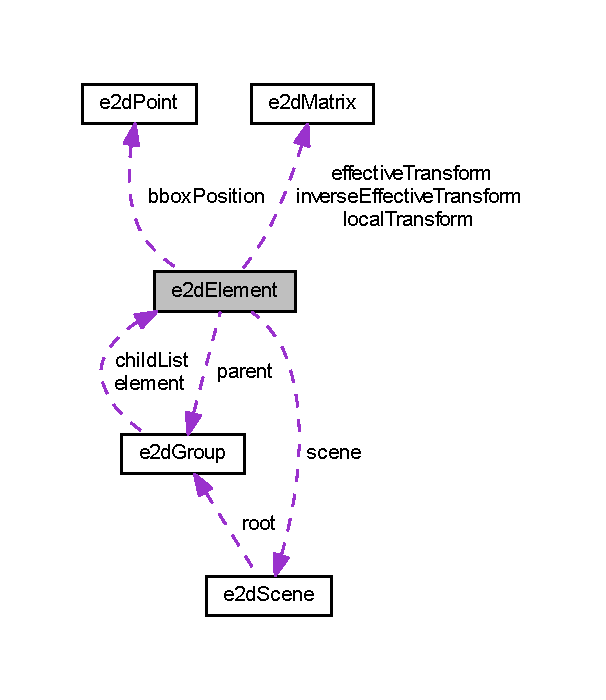
\includegraphics[width=291pt]{structe2d_element__coll__graph}
\end{center}
\end{figure}
\subsection*{Data Fields}
\begin{DoxyCompactItemize}
\item 
\hyperlink{structe2d_scene}{e2d\-Scene} $\ast$ \hyperlink{structe2d_element_a0ebd8fae058dd45496c86a2ca317ca9c}{scene}
\item 
\hyperlink{group__e2d_element_ga9bc8cfdec08c7e9069fc707ee456fd38}{e2d\-Element\-Type} \hyperlink{structe2d_element_a7df43d7f6c23b61b843acb56eb3ca19a}{type}
\item 
char $\ast$ \hyperlink{structe2d_element_aecb3b0d045ada529257a2fbf8f829599}{id}
\item 
unsigned int \hyperlink{structe2d_element_a300bb6cf5b184e200523e9bce8346dc4}{unique\-\_\-id}
\item 
\hyperlink{structe2d_matrix}{e2d\-Matrix} \hyperlink{structe2d_element_a52bda732df714953f93c1e6f5f7c7c93}{local\-Transform}
\item 
\hyperlink{structe2d_matrix}{e2d\-Matrix} \hyperlink{structe2d_element_a6c8e26945f09b5157e2111e42f99b879}{effective\-Transform}
\item 
\hyperlink{structe2d_matrix}{e2d\-Matrix} \hyperlink{structe2d_element_a5e6d7341f2dbef1923b0a3fcc13781c6}{inverse\-Effective\-Transform}
\item 
\hyperlink{structe2d_group}{e2d\-Group} $\ast$ \hyperlink{structe2d_element_a3e62eb2fbf1d6bc6d6fe549096a6cee9}{parent}
\item 
unsigned int \hyperlink{structe2d_element_a836181401227a3ca42da026a8d35e730}{attribute\-Num}
\item 
unsigned int \hyperlink{structe2d_element_a70d94929e3789bf7c019c939b0084985}{attribute\-Alloc}
\item 
char $\ast$$\ast$ \hyperlink{structe2d_element_af9b5d9dbbf270b6f92a3ee66ce1b47ac}{attribute\-Names}
\item 
char $\ast$$\ast$ \hyperlink{structe2d_element_ae8591ff93c366b4d66817a70f2d9f33e}{attribute\-Values}
\item 
float \hyperlink{structe2d_element_a6a1d9b223870deeaec7f5e8b23ca4b22}{bbox\-Width}
\item 
float \hyperlink{structe2d_element_a680d0d4219ac8720005c46b55a9676ae}{bbox\-Height}
\item 
\hyperlink{structe2d_point}{e2d\-Point} \hyperlink{structe2d_element_ac2c17ce4cba805b594b314a77923cbf5}{bbox\-Position}
\end{DoxyCompactItemize}


\subsection{Detailed Description}
The \hyperlink{structe2d_element}{e2d\-Element} struct is the base of all elements in the scene. Common scene information such as id, attribute values or transformations are saved in the \hyperlink{structe2d_element}{e2d\-Element} struct. You are not meant to instance this struct by itself. By creating other elements such as \hyperlink{structe2d_group}{e2d\-Group} or \hyperlink{structe2d_image}{e2d\-Image}, this struct will be automatically allocated in them. This \char`\"{}inheritance\char`\"{} is mimic'd by placing the \hyperlink{structe2d_element}{e2d\-Element} struct as the first element in structs which are meant to be \char`\"{}substructs\char`\"{} of it. 

\subsection{Field Documentation}
\hypertarget{structe2d_element_a70d94929e3789bf7c019c939b0084985}{\index{e2d\-Element@{e2d\-Element}!attribute\-Alloc@{attribute\-Alloc}}
\index{attribute\-Alloc@{attribute\-Alloc}!e2dElement@{e2d\-Element}}
\subsubsection[{attribute\-Alloc}]{\setlength{\rightskip}{0pt plus 5cm}unsigned int {\bf attribute\-Alloc}}}\label{structe2d_element_a70d94929e3789bf7c019c939b0084985}
Allocated size of \hyperlink{structe2d_group_a55f6dde874716dc99dcd270fc0999a01}{e2d\-Group\-::child\-List} \hypertarget{structe2d_element_af9b5d9dbbf270b6f92a3ee66ce1b47ac}{\index{e2d\-Element@{e2d\-Element}!attribute\-Names@{attribute\-Names}}
\index{attribute\-Names@{attribute\-Names}!e2dElement@{e2d\-Element}}
\subsubsection[{attribute\-Names}]{\setlength{\rightskip}{0pt plus 5cm}char$\ast$$\ast$ {\bf attribute\-Names}}}\label{structe2d_element_af9b5d9dbbf270b6f92a3ee66ce1b47ac}
Attribute names array, allocated size given by $<$ e2d\-Group\-::attribute\-Alloc. $<$ \begin{DoxySeeAlso}{See also}
\hyperlink{group__e2d_element_ga5cfa0a343d3dd1a30b0addc4ec6e7f88}{e2d\-Element\-Add\-Attribute()} 
\end{DoxySeeAlso}
\hypertarget{structe2d_element_a836181401227a3ca42da026a8d35e730}{\index{e2d\-Element@{e2d\-Element}!attribute\-Num@{attribute\-Num}}
\index{attribute\-Num@{attribute\-Num}!e2dElement@{e2d\-Element}}
\subsubsection[{attribute\-Num}]{\setlength{\rightskip}{0pt plus 5cm}unsigned int {\bf attribute\-Num}}}\label{structe2d_element_a836181401227a3ca42da026a8d35e730}
Number of attributes in \hyperlink{structe2d_element_af9b5d9dbbf270b6f92a3ee66ce1b47ac}{e2d\-Element\-::attribute\-Names} and $<$ \hyperlink{structe2d_element_ae8591ff93c366b4d66817a70f2d9f33e}{e2d\-Element\-::attribute\-Values}. \hypertarget{structe2d_element_ae8591ff93c366b4d66817a70f2d9f33e}{\index{e2d\-Element@{e2d\-Element}!attribute\-Values@{attribute\-Values}}
\index{attribute\-Values@{attribute\-Values}!e2dElement@{e2d\-Element}}
\subsubsection[{attribute\-Values}]{\setlength{\rightskip}{0pt plus 5cm}char$\ast$$\ast$ {\bf attribute\-Values}}}\label{structe2d_element_ae8591ff93c366b4d66817a70f2d9f33e}
Attribute values array, allocated size given by $<$ e2d\-Group\-::attribute\-Alloc. $<$ \begin{DoxySeeAlso}{See also}
\hyperlink{group__e2d_element_ga5cfa0a343d3dd1a30b0addc4ec6e7f88}{e2d\-Element\-Add\-Attribute()} 
\end{DoxySeeAlso}
\hypertarget{structe2d_element_a680d0d4219ac8720005c46b55a9676ae}{\index{e2d\-Element@{e2d\-Element}!bbox\-Height@{bbox\-Height}}
\index{bbox\-Height@{bbox\-Height}!e2dElement@{e2d\-Element}}
\subsubsection[{bbox\-Height}]{\setlength{\rightskip}{0pt plus 5cm}float {\bf bbox\-Height}}}\label{structe2d_element_a680d0d4219ac8720005c46b55a9676ae}
Bounding box height. $<$ \begin{DoxySeeAlso}{See also}
\hyperlink{group__e2d_element_ga94aa710b2da71af2091fe4d5b87ce47e}{e2d\-Element\-Calculate\-Bounding\-Box()} $<$ 

\hyperlink{group__e2d_element_ga36b01a888c97163c990e16d348aff61c}{e2d\-Element\-Center\-At\-B\-Box()} 
\end{DoxySeeAlso}
\hypertarget{structe2d_element_ac2c17ce4cba805b594b314a77923cbf5}{\index{e2d\-Element@{e2d\-Element}!bbox\-Position@{bbox\-Position}}
\index{bbox\-Position@{bbox\-Position}!e2dElement@{e2d\-Element}}
\subsubsection[{bbox\-Position}]{\setlength{\rightskip}{0pt plus 5cm}{\bf e2d\-Point} {\bf bbox\-Position}}}\label{structe2d_element_ac2c17ce4cba805b594b314a77923cbf5}
Bounding box position. $<$ \begin{DoxySeeAlso}{See also}
\hyperlink{group__e2d_element_ga94aa710b2da71af2091fe4d5b87ce47e}{e2d\-Element\-Calculate\-Bounding\-Box()} $<$ 

\hyperlink{group__e2d_element_ga36b01a888c97163c990e16d348aff61c}{e2d\-Element\-Center\-At\-B\-Box()} 
\end{DoxySeeAlso}
\hypertarget{structe2d_element_a6a1d9b223870deeaec7f5e8b23ca4b22}{\index{e2d\-Element@{e2d\-Element}!bbox\-Width@{bbox\-Width}}
\index{bbox\-Width@{bbox\-Width}!e2dElement@{e2d\-Element}}
\subsubsection[{bbox\-Width}]{\setlength{\rightskip}{0pt plus 5cm}float {\bf bbox\-Width}}}\label{structe2d_element_a6a1d9b223870deeaec7f5e8b23ca4b22}
Bounding box width. $<$ \begin{DoxySeeAlso}{See also}
\hyperlink{group__e2d_element_ga94aa710b2da71af2091fe4d5b87ce47e}{e2d\-Element\-Calculate\-Bounding\-Box()} $<$ 

\hyperlink{group__e2d_element_ga36b01a888c97163c990e16d348aff61c}{e2d\-Element\-Center\-At\-B\-Box()} 
\end{DoxySeeAlso}
\hypertarget{structe2d_element_a6c8e26945f09b5157e2111e42f99b879}{\index{e2d\-Element@{e2d\-Element}!effective\-Transform@{effective\-Transform}}
\index{effective\-Transform@{effective\-Transform}!e2dElement@{e2d\-Element}}
\subsubsection[{effective\-Transform}]{\setlength{\rightskip}{0pt plus 5cm}{\bf e2d\-Matrix} {\bf effective\-Transform}}}\label{structe2d_element_a6c8e26945f09b5157e2111e42f99b879}
Actual transform calculated applied here. $<$ \begin{DoxySeeAlso}{See also}
e2d\-Scene\-Calculate\-Effective\-Transforms() 
\end{DoxySeeAlso}
\hypertarget{structe2d_element_aecb3b0d045ada529257a2fbf8f829599}{\index{e2d\-Element@{e2d\-Element}!id@{id}}
\index{id@{id}!e2dElement@{e2d\-Element}}
\subsubsection[{id}]{\setlength{\rightskip}{0pt plus 5cm}char$\ast$ {\bf id}}}\label{structe2d_element_aecb3b0d045ada529257a2fbf8f829599}
I\-D taken from S\-V\-G \hypertarget{structe2d_element_a5e6d7341f2dbef1923b0a3fcc13781c6}{\index{e2d\-Element@{e2d\-Element}!inverse\-Effective\-Transform@{inverse\-Effective\-Transform}}
\index{inverse\-Effective\-Transform@{inverse\-Effective\-Transform}!e2dElement@{e2d\-Element}}
\subsubsection[{inverse\-Effective\-Transform}]{\setlength{\rightskip}{0pt plus 5cm}{\bf e2d\-Matrix} {\bf inverse\-Effective\-Transform}}}\label{structe2d_element_a5e6d7341f2dbef1923b0a3fcc13781c6}
Useful for point transformations. $<$ $<$ \begin{DoxySeeAlso}{See also}
\hyperlink{group__e2d_element_ga39dd883e42f609efba3f75300a29ff31}{e2d\-Element\-Get\-Local\-Position()} $<$ 

\hyperlink{group__e2d_element_ga9b85de42e52c0d89e82f9231ea923c8c}{e2d\-Element\-Get\-World\-Position()} $<$ 

\hyperlink{group__e2d_element_gab4e3f4eeba31c937a946f68617c5cb06}{e2d\-Element\-Get\-Relative\-Position()} $<$ 

\hyperlink{group__e2d_element_gac3ad9f8cdc0782378c9f2e93cb7da68f}{e2d\-Element\-Get\-Relative\-Point()} 
\end{DoxySeeAlso}
\hypertarget{structe2d_element_a52bda732df714953f93c1e6f5f7c7c93}{\index{e2d\-Element@{e2d\-Element}!local\-Transform@{local\-Transform}}
\index{local\-Transform@{local\-Transform}!e2dElement@{e2d\-Element}}
\subsubsection[{local\-Transform}]{\setlength{\rightskip}{0pt plus 5cm}{\bf e2d\-Matrix} {\bf local\-Transform}}}\label{structe2d_element_a52bda732df714953f93c1e6f5f7c7c93}
Local\-Transform taken from S\-V\-G \hypertarget{structe2d_element_a3e62eb2fbf1d6bc6d6fe549096a6cee9}{\index{e2d\-Element@{e2d\-Element}!parent@{parent}}
\index{parent@{parent}!e2dElement@{e2d\-Element}}
\subsubsection[{parent}]{\setlength{\rightskip}{0pt plus 5cm}{\bf e2d\-Group}$\ast$ {\bf parent}}}\label{structe2d_element_a3e62eb2fbf1d6bc6d6fe549096a6cee9}
parent of the element in the scene tree. \hypertarget{structe2d_element_a0ebd8fae058dd45496c86a2ca317ca9c}{\index{e2d\-Element@{e2d\-Element}!scene@{scene}}
\index{scene@{scene}!e2dElement@{e2d\-Element}}
\subsubsection[{scene}]{\setlength{\rightskip}{0pt plus 5cm}{\bf e2d\-Scene}$\ast$ {\bf scene}}}\label{structe2d_element_a0ebd8fae058dd45496c86a2ca317ca9c}
Belongs to this scene \hypertarget{structe2d_element_a7df43d7f6c23b61b843acb56eb3ca19a}{\index{e2d\-Element@{e2d\-Element}!type@{type}}
\index{type@{type}!e2dElement@{e2d\-Element}}
\subsubsection[{type}]{\setlength{\rightskip}{0pt plus 5cm}{\bf e2d\-Element\-Type} {\bf type}}}\label{structe2d_element_a7df43d7f6c23b61b843acb56eb3ca19a}
Used for reflection \hypertarget{structe2d_element_a300bb6cf5b184e200523e9bce8346dc4}{\index{e2d\-Element@{e2d\-Element}!unique\-\_\-id@{unique\-\_\-id}}
\index{unique\-\_\-id@{unique\-\_\-id}!e2dElement@{e2d\-Element}}
\subsubsection[{unique\-\_\-id}]{\setlength{\rightskip}{0pt plus 5cm}unsigned int {\bf unique\-\_\-id}}}\label{structe2d_element_a300bb6cf5b184e200523e9bce8346dc4}
unique id for this execution. $<$ (static int in \hyperlink{group__e2d_group_ga25406e9ff8a7746af03833e40ccf259a}{e2d\-Group\-Init()} ) 

The documentation for this struct was generated from the following file\-:\begin{DoxyCompactItemize}
\item 
C\-:/\-Users/\-Rui/\-Desktop/\-Ez2\-D\-S/\-Ez2\-D\-S/\-Ez2\-D\-S/\hyperlink{e2d_element_8h}{e2d\-Element.\-h}\end{DoxyCompactItemize}

\hypertarget{structe2d_group}{\section{e2d\-Group Struct Reference}
\label{structe2d_group}\index{e2d\-Group@{e2d\-Group}}
}


The e2d\-Struct is used to group elements in the scene, called childs. This struct is created from the \char`\"{}g\char`\"{} element in S\-V\-G. It \char`\"{}inherits\char`\"{} from \hyperlink{structe2d_element}{e2d\-Element} by placing it as the first element in the struct, if you typecast e2d\-Struct$\ast$ into e2d\-Element$\ast$, it will work thus mimicing inheritance in e.\-g. C++.  




{\ttfamily \#include $<$e2d\-Group.\-h$>$}



Collaboration diagram for e2d\-Group\-:\nopagebreak
\begin{figure}[H]
\begin{center}
\leavevmode
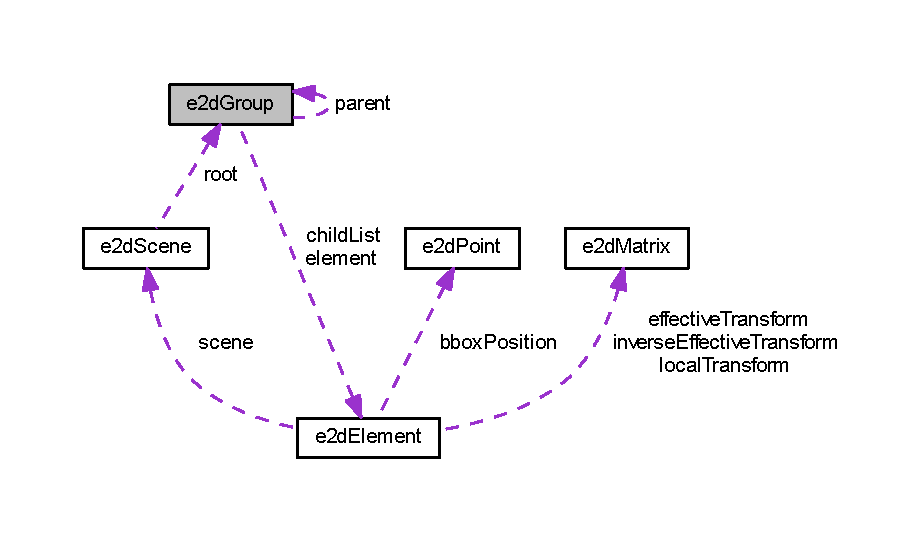
\includegraphics[width=350pt]{structe2d_group__coll__graph}
\end{center}
\end{figure}
\subsection*{Data Fields}
\begin{DoxyCompactItemize}
\item 
\hyperlink{structe2d_element}{e2d\-Element} \hyperlink{structe2d_group_a55bc7a3a0af41fba9e5b91f390c5928c}{element}
\item 
unsigned int \hyperlink{structe2d_group_a0af3697c2c9df6ed0ddd340cded35d65}{child\-Num}
\item 
\hyperlink{structe2d_element}{e2d\-Element} $\ast$$\ast$ \hyperlink{structe2d_group_a55f6dde874716dc99dcd270fc0999a01}{child\-List}
\item 
unsigned int \hyperlink{structe2d_group_a9c89d7cf35b835ef1917855c78a79cc5}{child\-List\-Alloc}
\end{DoxyCompactItemize}


\subsection{Detailed Description}
The e2d\-Struct is used to group elements in the scene, called childs. This struct is created from the \char`\"{}g\char`\"{} element in S\-V\-G. It \char`\"{}inherits\char`\"{} from \hyperlink{structe2d_element}{e2d\-Element} by placing it as the first element in the struct, if you typecast e2d\-Struct$\ast$ into e2d\-Element$\ast$, it will work thus mimicing inheritance in e.\-g. C++. 

\subsection{Field Documentation}
\hypertarget{structe2d_group_a55f6dde874716dc99dcd270fc0999a01}{\index{e2d\-Group@{e2d\-Group}!child\-List@{child\-List}}
\index{child\-List@{child\-List}!e2dGroup@{e2d\-Group}}
\subsubsection[{child\-List}]{\setlength{\rightskip}{0pt plus 5cm}{\bf e2d\-Element}$\ast$$\ast$ {\bf child\-List}}}\label{structe2d_group_a55f6dde874716dc99dcd270fc0999a01}
child list array, allocated size given by $<$ \hyperlink{structe2d_group_a9c89d7cf35b835ef1917855c78a79cc5}{e2d\-Group\-::child\-List\-Alloc}. $<$ \begin{DoxySeeAlso}{See also}
\hyperlink{group__e2d_group_ga6ae76730f78ad731621e9286a3980b8a}{e2d\-Group\-Add\-Child()} 
\end{DoxySeeAlso}
\hypertarget{structe2d_group_a9c89d7cf35b835ef1917855c78a79cc5}{\index{e2d\-Group@{e2d\-Group}!child\-List\-Alloc@{child\-List\-Alloc}}
\index{child\-List\-Alloc@{child\-List\-Alloc}!e2dGroup@{e2d\-Group}}
\subsubsection[{child\-List\-Alloc}]{\setlength{\rightskip}{0pt plus 5cm}unsigned int {\bf child\-List\-Alloc}}}\label{structe2d_group_a9c89d7cf35b835ef1917855c78a79cc5}
Allocated size of \hyperlink{structe2d_group_a55f6dde874716dc99dcd270fc0999a01}{e2d\-Group\-::child\-List} \hypertarget{structe2d_group_a0af3697c2c9df6ed0ddd340cded35d65}{\index{e2d\-Group@{e2d\-Group}!child\-Num@{child\-Num}}
\index{child\-Num@{child\-Num}!e2dGroup@{e2d\-Group}}
\subsubsection[{child\-Num}]{\setlength{\rightskip}{0pt plus 5cm}unsigned int {\bf child\-Num}}}\label{structe2d_group_a0af3697c2c9df6ed0ddd340cded35d65}
Number of children in e2d\-Group\-::child\-List\-Array \hypertarget{structe2d_group_a55bc7a3a0af41fba9e5b91f390c5928c}{\index{e2d\-Group@{e2d\-Group}!element@{element}}
\index{element@{element}!e2dGroup@{e2d\-Group}}
\subsubsection[{element}]{\setlength{\rightskip}{0pt plus 5cm}{\bf e2d\-Element} {\bf element}}}\label{structe2d_group_a55bc7a3a0af41fba9e5b91f390c5928c}
\hyperlink{structe2d_group}{e2d\-Group} inherits from \hyperlink{structe2d_element}{e2d\-Element}. Typecasting $<$ e2d\-Group$\ast$ to e2d\-Element$\ast$ will work. 

The documentation for this struct was generated from the following file\-:\begin{DoxyCompactItemize}
\item 
C\-:/\-Users/\-Rui/\-Desktop/\-Ez2\-D\-S/\-Ez2\-D\-S/\-Ez2\-D\-S/\hyperlink{e2d_group_8h}{e2d\-Group.\-h}\end{DoxyCompactItemize}

\hypertarget{structe2d_group_iterator}{\section{e2d\-Group\-Iterator Struct Reference}
\label{structe2d_group_iterator}\index{e2d\-Group\-Iterator@{e2d\-Group\-Iterator}}
}


Collaboration diagram for e2d\-Group\-Iterator\-:\nopagebreak
\begin{figure}[H]
\begin{center}
\leavevmode
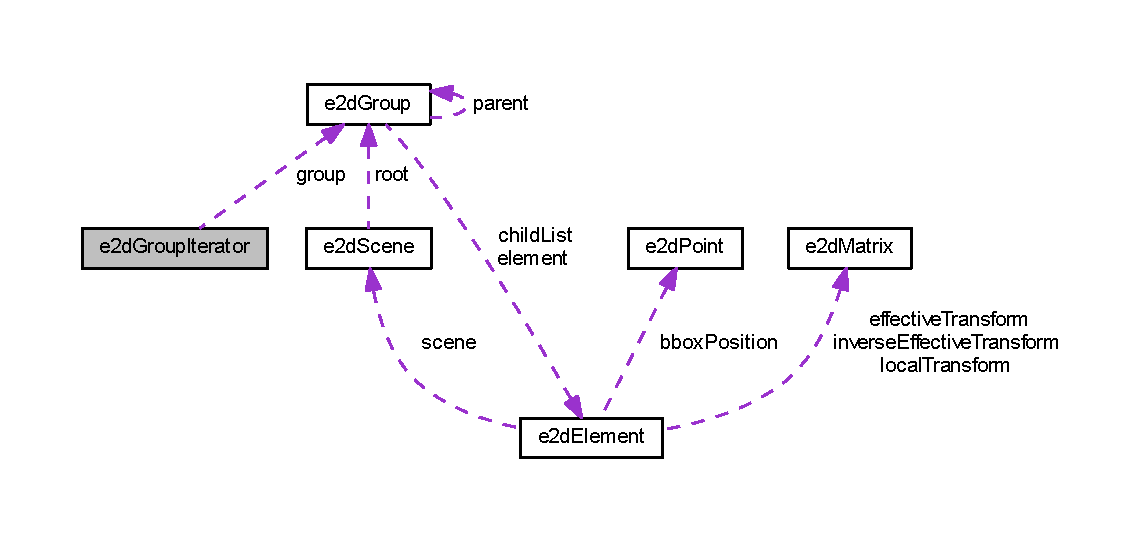
\includegraphics[width=350pt]{structe2d_group_iterator__coll__graph}
\end{center}
\end{figure}
\subsection*{Data Fields}
\begin{DoxyCompactItemize}
\item 
\hypertarget{structe2d_group_iterator_a13e9c2162587f7af49d2ceb78c380444}{\hyperlink{structe2d_group}{e2d\-Group} $\ast$ {\bfseries group}}\label{structe2d_group_iterator_a13e9c2162587f7af49d2ceb78c380444}

\item 
\hypertarget{structe2d_group_iterator_a932f59c8e81a171eb21af8d204d1c13d}{unsigned int {\bfseries current\-Index}}\label{structe2d_group_iterator_a932f59c8e81a171eb21af8d204d1c13d}

\end{DoxyCompactItemize}


The documentation for this struct was generated from the following file\-:\begin{DoxyCompactItemize}
\item 
C\-:/\-Users/\-Rui/\-Desktop/\-Ez2\-D\-S/\-Ez2\-D\-S/\-Ez2\-D\-S/e2d\-Group.\-h\end{DoxyCompactItemize}

\hypertarget{structe2d_image}{\section{e2d\-Image Struct Reference}
\label{structe2d_image}\index{e2d\-Image@{e2d\-Image}}
}


Collaboration diagram for e2d\-Image\-:\nopagebreak
\begin{figure}[H]
\begin{center}
\leavevmode
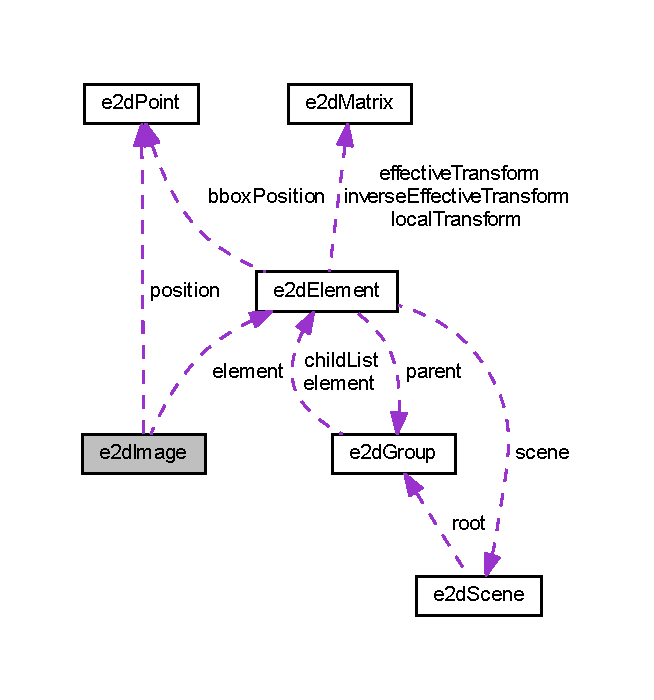
\includegraphics[width=314pt]{structe2d_image__coll__graph}
\end{center}
\end{figure}
\subsection*{Data Fields}
\begin{DoxyCompactItemize}
\item 
\hypertarget{structe2d_image_a55bc7a3a0af41fba9e5b91f390c5928c}{\hyperlink{structe2d_element}{e2d\-Element} {\bfseries element}}\label{structe2d_image_a55bc7a3a0af41fba9e5b91f390c5928c}

\item 
\hypertarget{structe2d_image_afa8983f25fd6aa6aca18feb07d8d2249}{\hyperlink{structe2d_point}{e2d\-Point} {\bfseries position}}\label{structe2d_image_afa8983f25fd6aa6aca18feb07d8d2249}

\item 
\hypertarget{structe2d_image_ae426f00e82704fa09578f5446e22d915}{float {\bfseries width}}\label{structe2d_image_ae426f00e82704fa09578f5446e22d915}

\item 
\hypertarget{structe2d_image_a48083b65ac9a863566dc3e3fff09a5b4}{float {\bfseries height}}\label{structe2d_image_a48083b65ac9a863566dc3e3fff09a5b4}

\item 
\hypertarget{structe2d_image_afb14ab23ba86115c3b01ad4122943f89}{char $\ast$ {\bfseries image\-Path}}\label{structe2d_image_afb14ab23ba86115c3b01ad4122943f89}

\end{DoxyCompactItemize}


The documentation for this struct was generated from the following file\-:\begin{DoxyCompactItemize}
\item 
C\-:/\-Users/\-Rui/\-Desktop/\-Ez2\-D\-S/\-Ez2\-D\-S/\-Ez2\-D\-S/e2d\-Image.\-h\end{DoxyCompactItemize}

\hypertarget{structe2d_matrix}{\section{e2d\-Matrix Struct Reference}
\label{structe2d_matrix}\index{e2d\-Matrix@{e2d\-Matrix}}
}
\subsection*{Data Fields}
\begin{DoxyCompactItemize}
\item 
\hypertarget{structe2d_matrix_ac06a92ccf2617d904678c51c6cf5a9bb}{float {\bfseries vals} \mbox{[}3\mbox{]}\mbox{[}3\mbox{]}}\label{structe2d_matrix_ac06a92ccf2617d904678c51c6cf5a9bb}

\end{DoxyCompactItemize}


The documentation for this struct was generated from the following file\-:\begin{DoxyCompactItemize}
\item 
C\-:/\-Users/\-Rui/\-Desktop/\-Ez2\-D\-S/\-Ez2\-D\-S/\-Ez2\-D\-S/e2d\-Matrix.\-h\end{DoxyCompactItemize}

\hypertarget{structe2d_path}{\section{e2d\-Path Struct Reference}
\label{structe2d_path}\index{e2d\-Path@{e2d\-Path}}
}


Collaboration diagram for e2d\-Path\-:\nopagebreak
\begin{figure}[H]
\begin{center}
\leavevmode
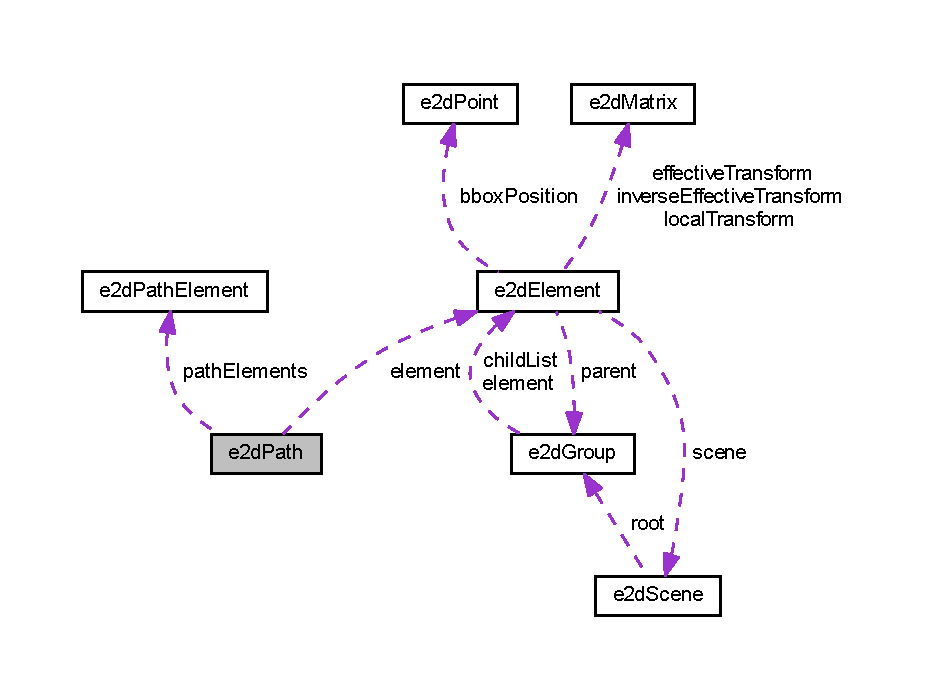
\includegraphics[width=350pt]{structe2d_path__coll__graph}
\end{center}
\end{figure}
\subsection*{Data Fields}
\begin{DoxyCompactItemize}
\item 
\hypertarget{structe2d_path_a55bc7a3a0af41fba9e5b91f390c5928c}{\hyperlink{structe2d_element}{e2d\-Element} {\bfseries element}}\label{structe2d_path_a55bc7a3a0af41fba9e5b91f390c5928c}

\item 
\hypertarget{structe2d_path_a225f71916c061d0c977a1e5fae371a99}{unsigned int {\bfseries path\-Elements\-Num}}\label{structe2d_path_a225f71916c061d0c977a1e5fae371a99}

\item 
\hypertarget{structe2d_path_ac0c8a45ff4f8d02e557fb33887743439}{\hyperlink{structe2d_path_element}{e2d\-Path\-Element} $\ast$$\ast$ {\bfseries path\-Elements}}\label{structe2d_path_ac0c8a45ff4f8d02e557fb33887743439}

\item 
\hypertarget{structe2d_path_a0922122c6ccf006fad850c6b30ae5328}{unsigned int {\bfseries path\-Elements\-Alloc}}\label{structe2d_path_a0922122c6ccf006fad850c6b30ae5328}

\end{DoxyCompactItemize}


The documentation for this struct was generated from the following file\-:\begin{DoxyCompactItemize}
\item 
C\-:/\-Users/\-Rui/\-Desktop/\-Ez2\-D\-S/\-Ez2\-D\-S/\-Ez2\-D\-S/e2d\-Path.\-h\end{DoxyCompactItemize}

\hypertarget{structe2d_path_curve}{\section{e2d\-Path\-Curve Struct Reference}
\label{structe2d_path_curve}\index{e2d\-Path\-Curve@{e2d\-Path\-Curve}}
}


Collaboration diagram for e2d\-Path\-Curve\-:\nopagebreak
\begin{figure}[H]
\begin{center}
\leavevmode
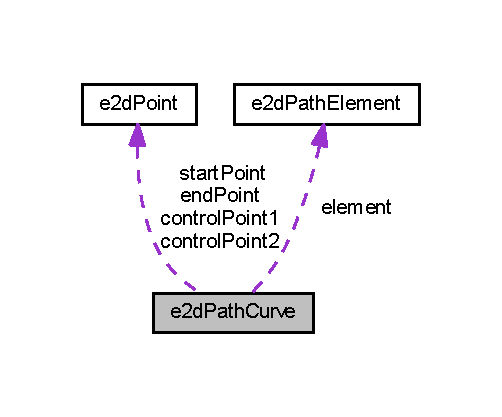
\includegraphics[width=241pt]{structe2d_path_curve__coll__graph}
\end{center}
\end{figure}
\subsection*{Data Fields}
\begin{DoxyCompactItemize}
\item 
\hypertarget{structe2d_path_curve_a88e514266530010a1a3b08198b3cc763}{\hyperlink{structe2d_path_element}{e2d\-Path\-Element} {\bfseries element}}\label{structe2d_path_curve_a88e514266530010a1a3b08198b3cc763}

\item 
\hypertarget{structe2d_path_curve_a96868a222a14861eb6e64214328c6159}{\hyperlink{structe2d_point}{e2d\-Point} {\bfseries start\-Point}}\label{structe2d_path_curve_a96868a222a14861eb6e64214328c6159}

\item 
\hypertarget{structe2d_path_curve_a5fe58a06185a33704c2cc77c8a58fb0d}{\hyperlink{structe2d_point}{e2d\-Point} {\bfseries control\-Point1}}\label{structe2d_path_curve_a5fe58a06185a33704c2cc77c8a58fb0d}

\item 
\hypertarget{structe2d_path_curve_a929324aa1e3527d71e312e5f80cb24db}{\hyperlink{structe2d_point}{e2d\-Point} {\bfseries control\-Point2}}\label{structe2d_path_curve_a929324aa1e3527d71e312e5f80cb24db}

\item 
\hypertarget{structe2d_path_curve_a0ae59a21d141722d36c0ebc740587f9d}{\hyperlink{structe2d_point}{e2d\-Point} {\bfseries end\-Point}}\label{structe2d_path_curve_a0ae59a21d141722d36c0ebc740587f9d}

\end{DoxyCompactItemize}


The documentation for this struct was generated from the following file\-:\begin{DoxyCompactItemize}
\item 
C\-:/\-Users/\-Rui/\-Desktop/\-Ez2\-D\-S/\-Ez2\-D\-S/\-Ez2\-D\-S/e2d\-Path.\-h\end{DoxyCompactItemize}

\hypertarget{structe2d_path_element}{\section{e2d\-Path\-Element Struct Reference}
\label{structe2d_path_element}\index{e2d\-Path\-Element@{e2d\-Path\-Element}}
}
\subsection*{Data Fields}
\begin{DoxyCompactItemize}
\item 
\hypertarget{structe2d_path_element_acb2ed01d1856b82777314d8eb8f66b01}{e2d\-Path\-Element\-Type {\bfseries type}}\label{structe2d_path_element_acb2ed01d1856b82777314d8eb8f66b01}

\item 
\hypertarget{structe2d_path_element_a88af317c0c6d0deb1aacb6cc1acd441d}{e2d\-Path\-Control {\bfseries control\-Type}}\label{structe2d_path_element_a88af317c0c6d0deb1aacb6cc1acd441d}

\end{DoxyCompactItemize}


The documentation for this struct was generated from the following file\-:\begin{DoxyCompactItemize}
\item 
C\-:/\-Users/\-Rui/\-Desktop/\-Ez2\-D\-S/\-Ez2\-D\-S/\-Ez2\-D\-S/e2d\-Path.\-h\end{DoxyCompactItemize}

\hypertarget{structe2d_path_element_iterator}{\section{e2d\-Path\-Element\-Iterator Struct Reference}
\label{structe2d_path_element_iterator}\index{e2d\-Path\-Element\-Iterator@{e2d\-Path\-Element\-Iterator}}
}


Collaboration diagram for e2d\-Path\-Element\-Iterator\-:\nopagebreak
\begin{figure}[H]
\begin{center}
\leavevmode
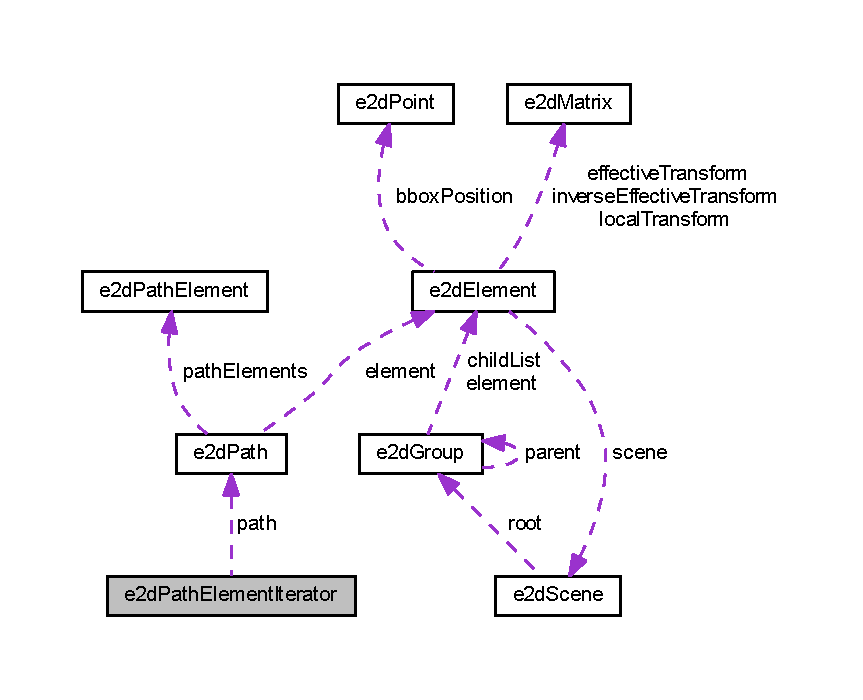
\includegraphics[width=350pt]{structe2d_path_element_iterator__coll__graph}
\end{center}
\end{figure}
\subsection*{Data Fields}
\begin{DoxyCompactItemize}
\item 
\hypertarget{structe2d_path_element_iterator_a318773d3a24970f193ecb5e2fcdce1a7}{\hyperlink{structe2d_path}{e2d\-Path} $\ast$ {\bfseries path}}\label{structe2d_path_element_iterator_a318773d3a24970f193ecb5e2fcdce1a7}

\item 
\hypertarget{structe2d_path_element_iterator_a932f59c8e81a171eb21af8d204d1c13d}{unsigned int {\bfseries current\-Index}}\label{structe2d_path_element_iterator_a932f59c8e81a171eb21af8d204d1c13d}

\end{DoxyCompactItemize}


The documentation for this struct was generated from the following file\-:\begin{DoxyCompactItemize}
\item 
C\-:/\-Users/\-Rui/\-Desktop/\-Ez2\-D\-S/\-Ez2\-D\-S/\-Ez2\-D\-S/e2d\-Path.\-h\end{DoxyCompactItemize}

\hypertarget{structe2d_path_point}{\section{e2d\-Path\-Point Struct Reference}
\label{structe2d_path_point}\index{e2d\-Path\-Point@{e2d\-Path\-Point}}
}


Collaboration diagram for e2d\-Path\-Point\-:\nopagebreak
\begin{figure}[H]
\begin{center}
\leavevmode
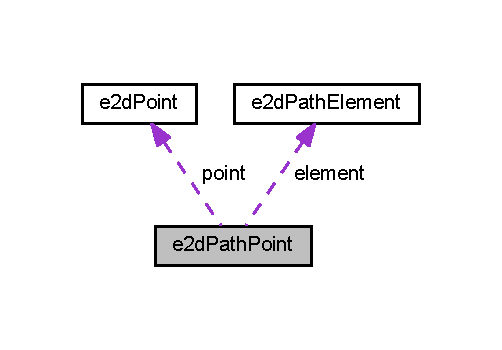
\includegraphics[width=241pt]{structe2d_path_point__coll__graph}
\end{center}
\end{figure}
\subsection*{Data Fields}
\begin{DoxyCompactItemize}
\item 
\hypertarget{structe2d_path_point_a88e514266530010a1a3b08198b3cc763}{\hyperlink{structe2d_path_element}{e2d\-Path\-Element} {\bfseries element}}\label{structe2d_path_point_a88e514266530010a1a3b08198b3cc763}

\item 
\hypertarget{structe2d_path_point_afff60c971a4d4728af80b4753d30c5bf}{\hyperlink{structe2d_point}{e2d\-Point} {\bfseries point}}\label{structe2d_path_point_afff60c971a4d4728af80b4753d30c5bf}

\end{DoxyCompactItemize}


The documentation for this struct was generated from the following file\-:\begin{DoxyCompactItemize}
\item 
C\-:/\-Users/\-Rui/\-Desktop/\-Ez2\-D\-S/\-Ez2\-D\-S/\-Ez2\-D\-S/e2d\-Path.\-h\end{DoxyCompactItemize}

\hypertarget{structe2d_point}{\section{e2d\-Point Struct Reference}
\label{structe2d_point}\index{e2d\-Point@{e2d\-Point}}
}


The \hyperlink{structe2d_point}{e2d\-Point} struct which contains two floats.  




{\ttfamily \#include $<$e2d\-Point.\-h$>$}

\subsection*{Data Fields}
\begin{DoxyCompactItemize}
\item 
float \hyperlink{structe2d_point_ad0da36b2558901e21e7a30f6c227a45e}{x}
\item 
float \hyperlink{structe2d_point_aa4f0d3eebc3c443f9be81bf48561a217}{y}
\end{DoxyCompactItemize}


\subsection{Detailed Description}
The \hyperlink{structe2d_point}{e2d\-Point} struct which contains two floats. 

\subsection{Field Documentation}
\hypertarget{structe2d_point_ad0da36b2558901e21e7a30f6c227a45e}{\index{e2d\-Point@{e2d\-Point}!x@{x}}
\index{x@{x}!e2dPoint@{e2d\-Point}}
\subsubsection[{x}]{\setlength{\rightskip}{0pt plus 5cm}float {\bf x}}}\label{structe2d_point_ad0da36b2558901e21e7a30f6c227a45e}
The X coordinate of the point \hypertarget{structe2d_point_aa4f0d3eebc3c443f9be81bf48561a217}{\index{e2d\-Point@{e2d\-Point}!y@{y}}
\index{y@{y}!e2dPoint@{e2d\-Point}}
\subsubsection[{y}]{\setlength{\rightskip}{0pt plus 5cm}float {\bf y}}}\label{structe2d_point_aa4f0d3eebc3c443f9be81bf48561a217}
The Y coordinate of the point 

The documentation for this struct was generated from the following file\-:\begin{DoxyCompactItemize}
\item 
C\-:/\-Users/\-Rui/\-Desktop/\-Ez2\-D\-S/\-Ez2\-D\-S/\-Ez2\-D\-S/\hyperlink{e2d_point_8h}{e2d\-Point.\-h}\end{DoxyCompactItemize}

\hypertarget{structe2d_scene}{\section{e2d\-Scene Struct Reference}
\label{structe2d_scene}\index{e2d\-Scene@{e2d\-Scene}}
}


Collaboration diagram for e2d\-Scene\-:\nopagebreak
\begin{figure}[H]
\begin{center}
\leavevmode
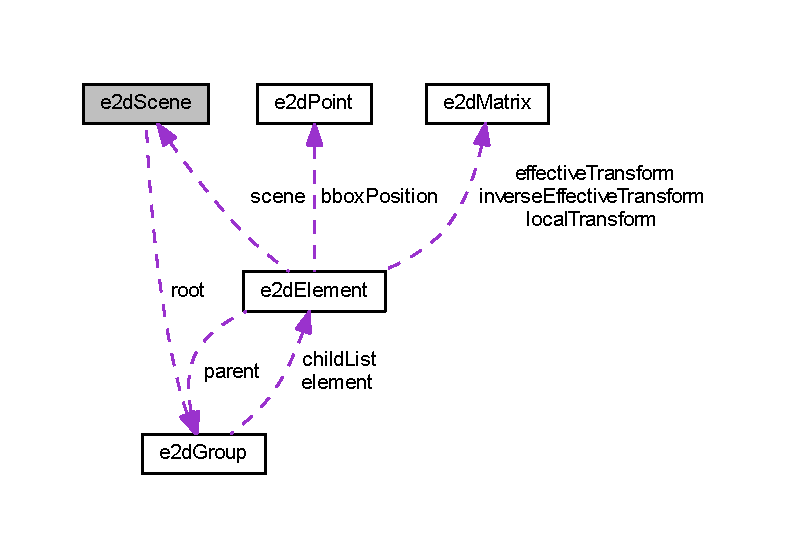
\includegraphics[width=350pt]{structe2d_scene__coll__graph}
\end{center}
\end{figure}
\subsection*{Data Fields}
\begin{DoxyCompactItemize}
\item 
\hypertarget{structe2d_scene_aa5444ac46bf18449921a4094bcadde1c}{\hyperlink{structe2d_group}{e2d\-Group} $\ast$ {\bfseries root}}\label{structe2d_scene_aa5444ac46bf18449921a4094bcadde1c}

\end{DoxyCompactItemize}


The documentation for this struct was generated from the following file\-:\begin{DoxyCompactItemize}
\item 
C\-:/\-Users/\-Rui/\-Desktop/\-Ez2\-D\-S/\-Ez2\-D\-S/\-Ez2\-D\-S/e2d\-Scene.\-h\end{DoxyCompactItemize}

\chapter{File Documentation}
\hypertarget{e2d_element_8h}{\section{C\-:/\-Users/\-Rui/\-Desktop/\-Ez2\-D\-S/\-Ez2\-D\-S/\-Ez2\-D\-S/e2d\-Element.h File Reference}
\label{e2d_element_8h}\index{C\-:/\-Users/\-Rui/\-Desktop/\-Ez2\-D\-S/\-Ez2\-D\-S/\-Ez2\-D\-S/e2d\-Element.\-h@{C\-:/\-Users/\-Rui/\-Desktop/\-Ez2\-D\-S/\-Ez2\-D\-S/\-Ez2\-D\-S/e2d\-Element.\-h}}
}


File which contains the \hyperlink{structe2d_element}{e2d\-Element} struct and its \char`\"{}methods\char`\"{}.  


{\ttfamily \#include \char`\"{}Ez2\-D\-S.\-h\char`\"{}}\\*
{\ttfamily \#include \char`\"{}e2d\-Matrix.\-h\char`\"{}}\\*
{\ttfamily \#include \char`\"{}e2d\-Point.\-h\char`\"{}}\\*
Include dependency graph for e2d\-Element.\-h\-:
\nopagebreak
\begin{figure}[H]
\begin{center}
\leavevmode
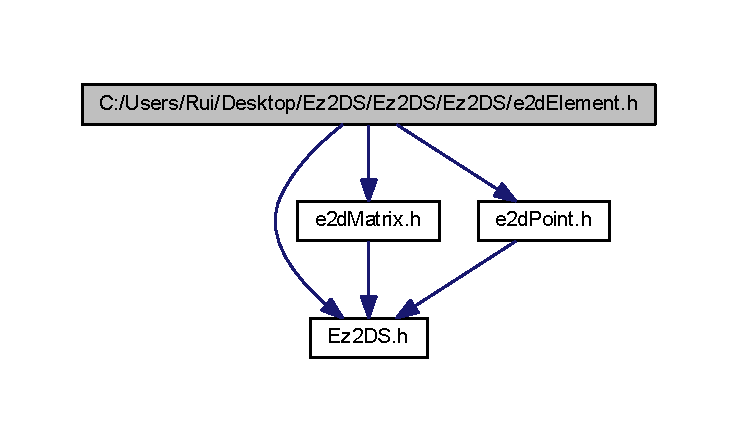
\includegraphics[width=350pt]{e2d_element_8h__incl}
\end{center}
\end{figure}
This graph shows which files directly or indirectly include this file\-:
\nopagebreak
\begin{figure}[H]
\begin{center}
\leavevmode
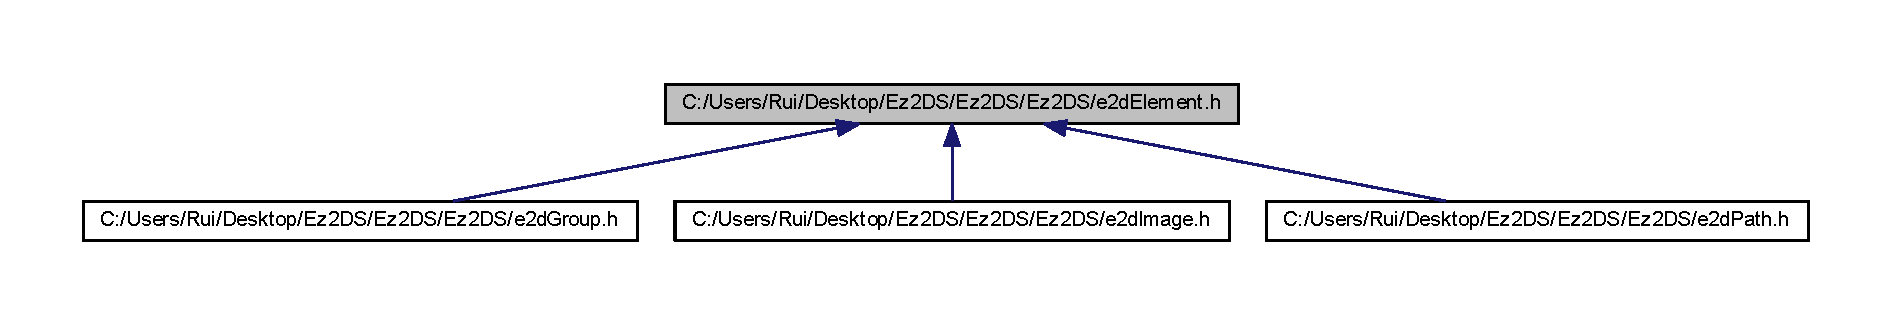
\includegraphics[width=350pt]{e2d_element_8h__dep__incl}
\end{center}
\end{figure}
\subsection*{Data Structures}
\begin{DoxyCompactItemize}
\item 
struct \hyperlink{structe2d_element}{e2d\-Element}
\begin{DoxyCompactList}\small\item\em The \hyperlink{structe2d_element}{e2d\-Element} struct is the base of all elements in the scene. Common scene information such as id, attribute values or transformations are saved in the \hyperlink{structe2d_element}{e2d\-Element} struct. You are not meant to instance this struct by itself. By creating other elements such as \hyperlink{structe2d_group}{e2d\-Group} or \hyperlink{structe2d_image}{e2d\-Image}, this struct will be automatically allocated in them. This \char`\"{}inheritance\char`\"{} is mimic'd by placing the \hyperlink{structe2d_element}{e2d\-Element} struct as the first element in structs which are meant to be \char`\"{}substructs\char`\"{} of it. \end{DoxyCompactList}\end{DoxyCompactItemize}
\subsection*{Typedefs}
\begin{DoxyCompactItemize}
\item 
\hypertarget{group__e2d_element_ga13e962cd8fa5eaa7d4bec3fc7d774d59}{typedef enum \hyperlink{group__e2d_element_ga9bc8cfdec08c7e9069fc707ee456fd38}{e2d\-Element\-Type} \hyperlink{group__e2d_element_ga13e962cd8fa5eaa7d4bec3fc7d774d59}{e2d\-Element\-Type}}\label{group__e2d_element_ga13e962cd8fa5eaa7d4bec3fc7d774d59}

\begin{DoxyCompactList}\small\item\em The e2d\-Element\-Type enum defines the possible \char`\"{}substructs\char`\"{} of \hyperlink{structe2d_element}{e2d\-Element}. This is used for reflection. \end{DoxyCompactList}\end{DoxyCompactItemize}
\subsection*{Enumerations}
\begin{DoxyCompactItemize}
\item 
enum \hyperlink{group__e2d_element_ga9bc8cfdec08c7e9069fc707ee456fd38}{e2d\-Element\-Type} \{ {\bfseries E2\-D\-\_\-\-G\-R\-O\-U\-P}, 
{\bfseries E2\-D\-\_\-\-P\-A\-T\-H}, 
{\bfseries E2\-D\-\_\-\-I\-M\-A\-G\-E}
 \}
\begin{DoxyCompactList}\small\item\em The e2d\-Element\-Type enum defines the possible \char`\"{}substructs\char`\"{} of \hyperlink{structe2d_element}{e2d\-Element}. This is used for reflection. \end{DoxyCompactList}\end{DoxyCompactItemize}
\subsection*{Functions}
\begin{DoxyCompactItemize}
\item 
void \hyperlink{group__e2d_element_ga8734d10ef40a380dfc51bfe1790a92a7}{e2d\-Element\-Init} (\hyperlink{structe2d_element}{e2d\-Element} $\ast$element, \hyperlink{group__e2d_element_ga9bc8cfdec08c7e9069fc707ee456fd38}{e2d\-Element\-Type} type, const \hyperlink{structe2d_scene}{e2d\-Scene} $\ast$scene)
\begin{DoxyCompactList}\small\item\em Called by the create methods of structs which inherit \hyperlink{structe2d_element}{e2d\-Element} (e.\-g. e2d\-Group\-Create). Will initialize all members of the struct with the parameters of this method and with default values on everything else. \end{DoxyCompactList}\item 
void \hyperlink{group__e2d_element_ga214c437a16fe6f3fc795539f851a2019}{e2d\-Element\-Destroy} (\hyperlink{structe2d_element}{e2d\-Element} $\ast$elem)
\begin{DoxyCompactList}\small\item\em Will check the type member of elem and call the appropriate destructor (e.\-g. e2d\-Group\-Destroy()) \end{DoxyCompactList}\item 
void \hyperlink{group__e2d_element_gae8da5104d70a09549ca74044dda8313c}{e2d\-Element\-Free\-Members} (\hyperlink{structe2d_element}{e2d\-Element} $\ast$elem)
\begin{DoxyCompactList}\small\item\em Will free all the allocated memory inside the \hyperlink{structe2d_element}{e2d\-Element} struct pointed by elem. \end{DoxyCompactList}\item 
void \hyperlink{group__e2d_element_ga5cfa0a343d3dd1a30b0addc4ec6e7f88}{e2d\-Element\-Add\-Attribute} (\hyperlink{structe2d_element}{e2d\-Element} $\ast$elem, const char $\ast$name, const char $\ast$value)
\begin{DoxyCompactList}\small\item\em Will add an attribute to the element. Increases the size of the array if necessary. \end{DoxyCompactList}\item 
const char $\ast$ \hyperlink{group__e2d_element_gac32ea8a33b317fc014929102d64ac157}{e2d\-Element\-Get\-Attribute} (\hyperlink{structe2d_element}{e2d\-Element} $\ast$elem, const char $\ast$name)
\begin{DoxyCompactList}\small\item\em Returns the value of an attribute with a given name. \end{DoxyCompactList}\item 
\hyperlink{structe2d_point}{e2d\-Point} \hyperlink{group__e2d_element_ga39dd883e42f609efba3f75300a29ff31}{e2d\-Element\-Get\-Local\-Position} (const \hyperlink{structe2d_element}{e2d\-Element} $\ast$elem)
\begin{DoxyCompactList}\small\item\em Returns the position of the element, taken from the local\-Transform. \end{DoxyCompactList}\item 
\hyperlink{structe2d_point}{e2d\-Point} \hyperlink{group__e2d_element_ga9b85de42e52c0d89e82f9231ea923c8c}{e2d\-Element\-Get\-World\-Position} (const \hyperlink{structe2d_element}{e2d\-Element} $\ast$elem)
\begin{DoxyCompactList}\small\item\em U\-N\-T\-E\-S\-T\-E\-D Will get the local position (\hyperlink{group__e2d_element_ga39dd883e42f609efba3f75300a29ff31}{e2d\-Element\-Get\-Local\-Position()}) and multiply it by the inverse\-Effective\-Transform and obtain the world position. Needs effective transformations to be calculated ( e2d\-Scene\-Calculate\-Effective\-Transforms() has been called) \end{DoxyCompactList}\item 
\hyperlink{structe2d_point}{e2d\-Point} \hyperlink{group__e2d_element_gab4e3f4eeba31c937a946f68617c5cb06}{e2d\-Element\-Get\-Relative\-Position} (const \hyperlink{structe2d_element}{e2d\-Element} $\ast$elem, const \hyperlink{structe2d_element}{e2d\-Element} $\ast$relative\-To)
\begin{DoxyCompactList}\small\item\em U\-N\-T\-E\-S\-T\-E\-D Will get the relative transformation by multiplying the effective transform of elem with the inverse effective transform of relative\-To. The multiply it with the local position of elem (\hyperlink{group__e2d_element_ga39dd883e42f609efba3f75300a29ff31}{e2d\-Element\-Get\-Local\-Position()}). Needs effective transformations to be calculated (e2d\-Scene\-Calculate\-Effective\-Transforms() has been called) \end{DoxyCompactList}\item 
\hyperlink{structe2d_point}{e2d\-Point} \hyperlink{group__e2d_element_gac3ad9f8cdc0782378c9f2e93cb7da68f}{e2d\-Element\-Get\-Relative\-Point} (const \hyperlink{structe2d_element}{e2d\-Element} $\ast$elem, const \hyperlink{structe2d_element}{e2d\-Element} $\ast$relative\-To, const \hyperlink{structe2d_point}{e2d\-Point} $\ast$point)
\begin{DoxyCompactList}\small\item\em U\-N\-T\-E\-S\-T\-E\-D Will get the relative transformation by multiplying the effective transform of elem with the inverse effective transform of relative\-To. The multiply it with point. Needs effective transformations to be calculated (e2d\-Scene\-Calculate\-Effective\-Transforms() has been called) \end{DoxyCompactList}\item 
void \hyperlink{group__e2d_element_ga94aa710b2da71af2091fe4d5b87ce47e}{e2d\-Element\-Calculate\-Bounding\-Box} (\hyperlink{structe2d_element}{e2d\-Element} $\ast$elem)
\begin{DoxyCompactList}\small\item\em Will check type and calculate the appropriate method (e.\-g. e2d\-Group\-Calculate\-Bounding\-Box()) \end{DoxyCompactList}\item 
void \hyperlink{group__e2d_element_ga36b01a888c97163c990e16d348aff61c}{e2d\-Element\-Center\-At\-B\-Box} (\hyperlink{structe2d_element}{e2d\-Element} $\ast$elem, float tx, float ty)
\begin{DoxyCompactList}\small\item\em Needs bounding box to have been calculated. Will check type and calculate the appropriate method (e.\-g. e2d\-Group\-Center\-At\-B\-Box()). (tx, ty) will define where in the bounding box, the element will be centered, e.\-g. (0,0, will center on the top left corner, (0.\-5, 0.\-5) will center on the center of the bbox. \end{DoxyCompactList}\end{DoxyCompactItemize}


\subsection{Detailed Description}
File which contains the \hyperlink{structe2d_element}{e2d\-Element} struct and its \char`\"{}methods\char`\"{}. \begin{DoxyAuthor}{Author}
Rui (\href{mailto:ruir2c@gmail.com}{\tt ruir2c@gmail.\-com})
\end{DoxyAuthor}
\begin{DoxyDate}{Date}
February, 2012 
\end{DoxyDate}

\printindex
\end{document}
